%%%%%%%%%%%%%%%%%%%%%%%%%%%%%%%%%%%%%%%%%
% Medium Length Professional CV
% LaTeX Template
% Version 2.0 (8/5/13)
%
% This template has been downloaded from:
% http://www.LaTeXTemplates.com
%
% Original author:
% Trey Hunner (http://www.treyhunner.com/)
%
% Important note:
% This template requires the resume.cls file to be in the same directory as the
% .tex file. The resume.cls file provides the resume style used for structuring the
% document.
%
%%%%%%%%%%%%%%%%%%%%%%%%%%%%%%%%%%%%%%%%%

%----------------------------------------------------------------------------------------
%	PACKAGES AND OTHER DOCUMENT CONFIGURATIONS
%----------------------------------------------------------------------------------------

\documentclass{resume} % Use the custom resume.cls style

\usepackage[UTF8]{ctex}
\usepackage[left=0.75in,top=0.6in,right=0.75in,bottom=0.6in]{geometry} % Document margins
\newcommand{\tab}[1]{\hspace{.2667\textwidth}\rlap{#1}}
\newcommand{\itab}[1]{\hspace{0em}\rlap{#1}}

\begin{document}

%%%%%%%%%%%%%%% ENTÊTE %%%%%%%%%%%%%%%
\begin{wrapfigure}[0]{r}[0pt]{0pt}
\vspace{-12pt}
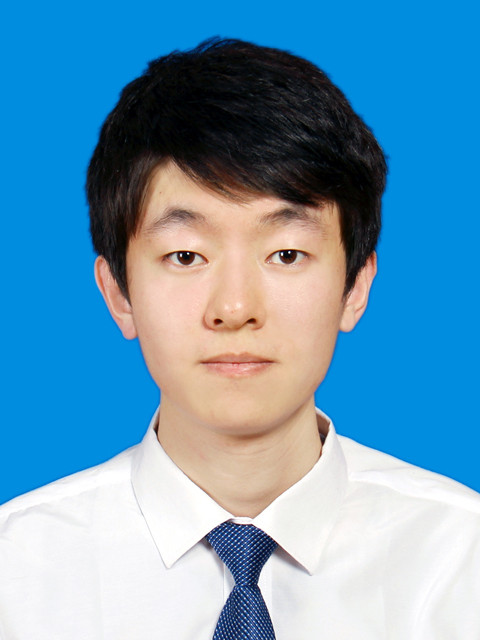
\includegraphics[scale=0.8]{fuliyu.jpg}
\end{wrapfigure}

\fontsize{20pt}{0pt}\selectfont
\bf{傅礼玉}

\normalfont
\fontsize{12pt}{14pt}\selectfont
哈尔滨工业大学,计算机科学与技术,硕士\\
研究方向:无线传感网络\\
1098356354@qq.com\\
(+86)15636828276\\
{\bf\Large\rmfamily    意向岗位:JAVA研发实习生}
\vspace{8pt}
%%%%%%%%%%%%%%% ENTÊTE %%%%%%%%%%%%%%%


%----------------------------------------------------------------------------------------
%	EDUCATION SECTION
%----------------------------------------------------------------------------------------

\begin{rSection}{教育背景}

{\bf (高中)山东省齐河县第一中学} \hfill {\em 2011.9 - 2014.6} 
\\ 全国青少年信息学奥林匹克联赛二等奖 \hfill {\em 2012.11/2013.11}
\\{\bf (本科)哈尔滨工业大学,计算机科学与技术} \hfill {\em 2014.9 - 2018.6} 
\\ 一等奖学金、三好学生、优秀毕业生、免试攻读研究生 \hfill {\em 专业课成绩:平均92}
\\ 黑龙江省大学生程序设计竞赛二等奖 \hfill {\em 2015.11}
\\{\bf (交换)台湾中正大学,资讯工程学系} \hfill {\em 2016.9 - 2017.1} 
\\{\bf (硕士)哈尔滨工业大学,计算机科学与技术} \hfill {\em 2018.9 - 2020.6} 
\\ 一等奖学金
%Minor in Linguistics \smallskip \\
%Member of Eta Kappa Nu \\
%Member of Upsilon Pi Epsilon \\


\end{rSection}
%----------------------------------------------------------------------------------------
%	TECHNICAL STRENGTHS SECTION
%----------------------------------------------------------------------------------------

\begin{rSection}{技能}

\begin{tabular}{ @{} >{\bfseries}l @{\hspace{6ex}} l }
熟练使用Python、C/C++\\
熟悉常用数据结构与算法\\
熟悉计算机网络、操作系统、体系结构、数据库等 \\
\end{tabular}

\end{rSection}

%----------------------------------------------------------------------------------------
%	WORK EXPERIENCE SECTION
%----------------------------------------------------------------------------------------

\begin{rSection}{实习经验}

\begin{rSubsection}{上海快仓}{2018.3 - 2018.5}{机器人控制系统部门}{}
\item 解决菜鸟网络无锡猫超仓网络问题(大量AGV漫游速度慢,掉线问题严重,严重影响正常业务):分析产生该问题的原因,调研学界和工业界对漫游问题的解决方案,创造性地将多路径TCP(MPTCP)技术应用于该项目,完美低成本地解决了网络问题,保证了仓库项目能按时验收。
\item 维护AGV中agent代码,调研测试自动化运维工具saltstack(类似于staragent)。
\end{rSubsection}


%------------------------------------------------

\begin{rSubsection}{字节跳动}{2018.7 - 2018.8}{效率工程-安全审计部门}{}
\item 效率工程内部堡垒机中的权限管理系统:使用Python/Flask/Docker/Html/Redis实现。
\item 效率工程内部堡垒机中的日志审计系统:修复显示客户端数量与实际客户端数量不一致、Kafka消费中断等若干BUG。
\item 为Lark服务器中Redis集群增加systemd服务。
\end{rSubsection}

\end{rSection}


%	EXAMPLE SECTION
%----------------------------------------------------------------------------------------

\begin{rSection}{学校项目}

\begin{rSubsection}{使用Scrapy框架爬取Google Scholar}{2016.10 - 2016.11}{}{}
\item 使用Python的Scrapy框架爬取了谷歌学术中的人员信息
\end{rSubsection}

%------------------------------------------------

\begin{rSubsection}{面向 AGV 近场通信的时间同步技术与设备驱动研究}{2017.10 - 2018.5}{}{}
\item IEEE 802.15.4通信协议、数据链路层的TDMA调度、CC2650驱动
\end{rSubsection}

%------------------------------------------------

\begin{rSubsection}{基于UWB的AGV定位、安全避让及通信方案}{2018.10 - 2019.3}{}{}
\item UWB通信测距、TDOA3定位算法、IEEE 802.15.4通信协议
\end{rSubsection}


%------------------------------------------------

\begin{rSubsection}{面向延迟敏感应用的MPTCP优化}{2019.4 - 2020.5}{}{}
\item 对所处网络环境不稳定但对延迟敏感的应用(比如AGV),MPTCP默认的拥塞控制和流量调度方式不尽如人意,利用跨层的方法对MPTCP的拥塞控制和流量调度方式进行优化
\end{rSubsection}

\end{document}
